% !TeX root = ../main.tex

\chapter{需求分析}
本章在上一章介绍的DNNCL深度学习计算库上测试不同的神经网络,探究运行时的状态,从而找到运行时优化的切入点。从需要实现什么入手,对本系统的需求进行分析和整理,确定本系统需要实现哪些功能以及需要满足哪些非功能性需求。然后将需求逐步求精和细化,分析各种可能的解法,并且分配给各个软件元素。

\section{需求挖掘}
本系统的主要目标是优化深度学习库的运行时过程,而运行时优化少不了对热点路径的探测和优化。通过在DNNCL库上运行经典神经网络,对运行时各个阶段的时间进行统计分析。包括拷贝输入输出时间、动态编译时间、加载Kernel的时间、IPU执行计算的时间。输入输出时间代表将数据输入数据从主机端考入到设备端和将结果从设备端拷出的时间;动态编译时间指的是从深度学习库拿到用户搭建的计算图后编译生成Kernel的时间;加载Kernel的时间指的是将编译好的Kernel从CPU端加载到设备端所用的时间;IPU执行计算的时间指的是启动IPU执行推理过程的时间。统计发现,绝大多数网络中,动态编译时间的开销占到了整个推理过程的99\%左右。也就是说动态编译的时间的占了整个推理时间的大头,所以想要增加神经网络的表现性能,可以将目标放在优化编译阶段。

由于DNNCL是由C和C++语言实现,C/C++程序是静态编译优化的典型代表,并且静态优化技术的成熟,使得静态优化对程序性能提升的空间越来越小。所以这里考虑用动态重编译技术来优化编译过程。结合神经网络应用的使用场景不难发现,一个相同的神经网络往往在短时间内被多次使用。而现在的模式下,每运行一次神经网络就会重新编译生成一次指令。每次都会花费很多时间在编译指令上,特别是在一些端设备上,长时间的等待是无法接受的。因此可以想办法优化编译的过程,避免相同神经网络的重复编译过程,减少调用同一程序带来的编译开销。
另外由于神经网络大多结构相同,针对不同的应用场景只是只有权值等数据发生了变化。如果有一份编译好的指令,支持动态更新里面的静态数据,那也可以省略掉重复编译的开销。

随着卷积神经网络模型堆叠的层数越来越多,网络模型的权重参数数量也随之增长,并且现在神经网络的权值数据大部分是用单精度4字节的float32或者双精度8字节的float64表示,所以网络模型存储体积越来越大。如果能降低模型的存储空间将更有助于将神经网络模型部署到通用的嵌入式移动平台。

\section {功能性需求}
从挖掘的需求分析,要避免重复编译带来的开销,应该将编译好的指令缓存起来。要想实现指令缓存,本优化系统则应该具备以下功能:
\begin{enumerate}
  \item 编译入口接收到的是用户构建的计算图,所以应该具有保存计算图、计算图识别的功能。
  \item 想要避免重复编译,则要想办法保存编译好的指令并且之后能解析指令文件,所以应该具有指令保存、指令加载的功能。
  \item 二进制机器代码是和硬件的驱动版本相关的,当驱动更新时,二进制代码也会发生变化,所以还应该就有向前兼容性
  \item 缓存的指令占用存储空间,不能无限制的增长,因此需要设置存储上限和合理的查找和替换策略。
\end{enumerate}

想要实现静态数据的更新,不仅需要识别出静态数据发生了变化,还需要识别出哪个静态数据发生了变化。所以应该就有静态数据标识,静态数据对比,静态数据替换的功能。

为了降低模型的存储空间达到模型压缩加速的目的,可以对参数进行量化。参数量化可以利用定点数表示浮点数的方式来实现,用1字节的int8来表示4字节的float32能节省大约4倍的存储空间。量化的过程中会带来一定的精度损失,但是可以减少存储空间、加速计算,带来性能方面的大幅提升。结合以上的分析,得到图~\ref{fig:user-need}所示用例图。

\begin{figure}[htb]
  \centering
  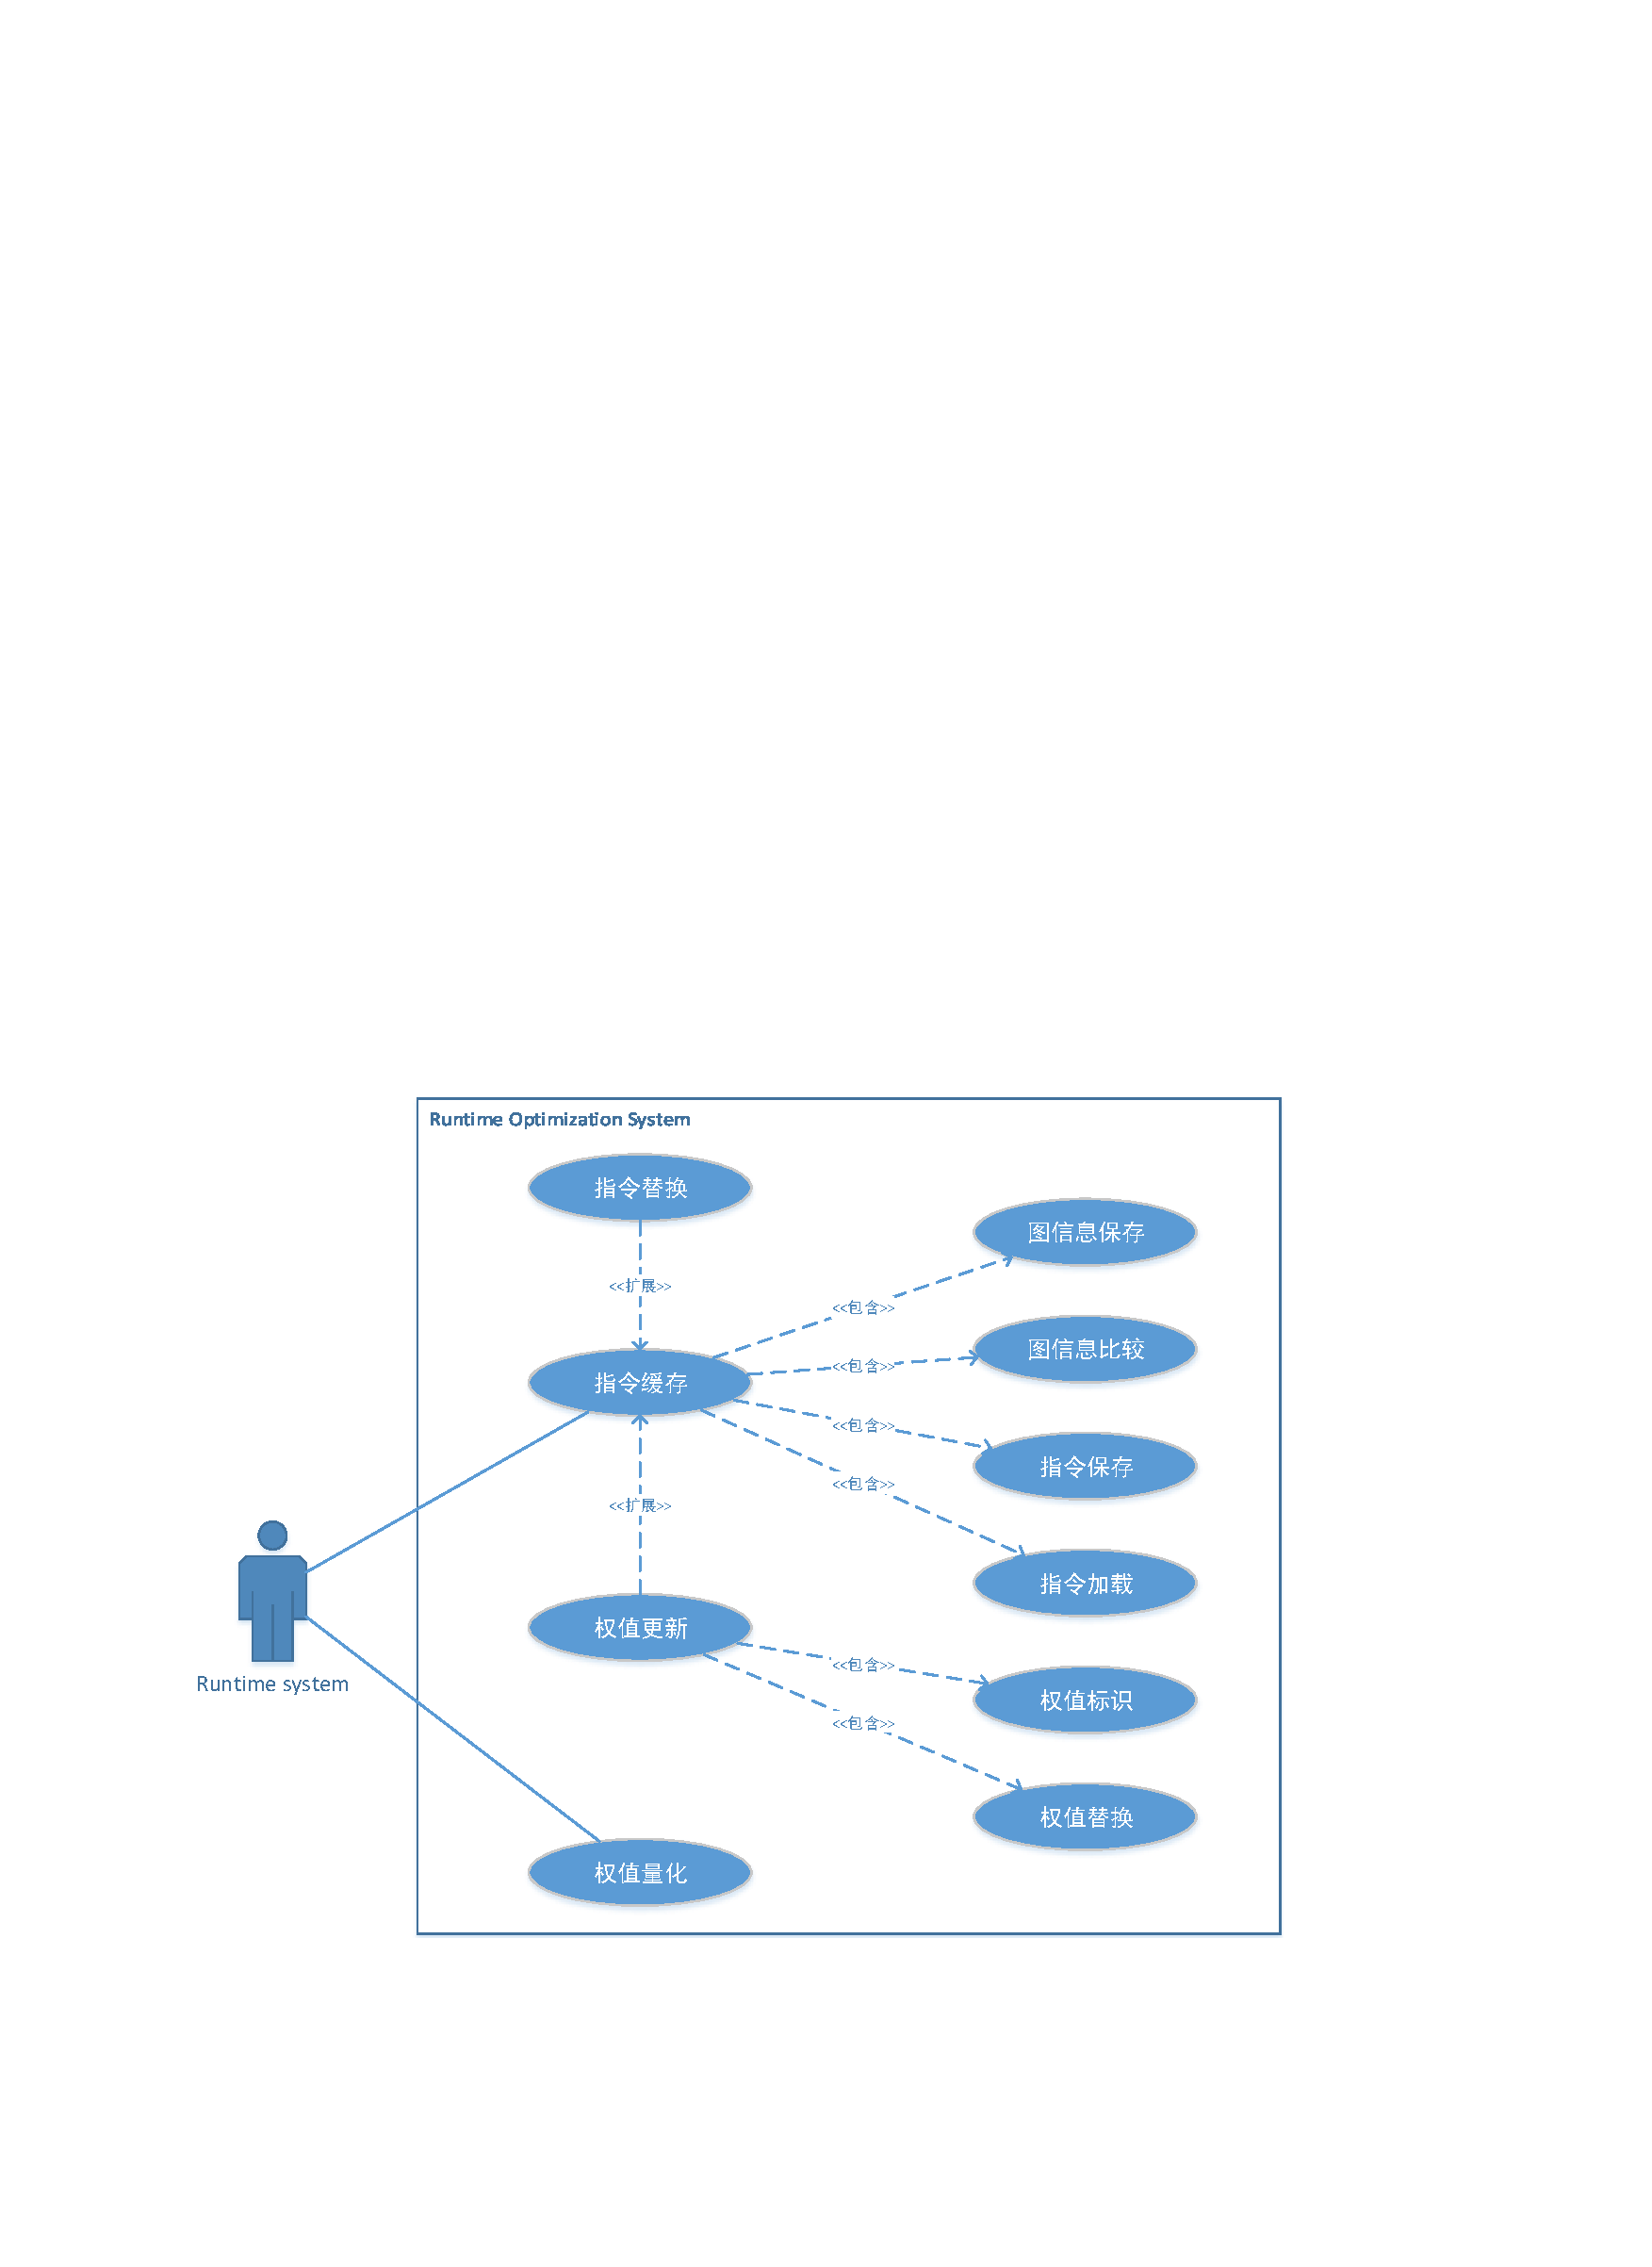
\includegraphics[width=0.6\textwidth]{user_need.pdf}
  \caption{运行时优化系统用例图}
  \label{fig:user-need}
\end{figure}

运行时优化系统属于对运行时的优化,对外用户不可见,通过特定的方式是功能生效。运行时优化系统应该具备以下功能:
\begin{enumerate}
  \item 指令缓存:指令缓存的功能中包含四个必不可少的功能,计算图信息保存、计算图信息比较、指令保存以及指令加载,有两个拓展功能,指令替换和权值更新。当缓存空间已满时需要用到指令替换功能,当计算图结构相同而权值信息不同时需要用到权值更新功能。权值更新的实现必须依赖权值标识和权值替换。
  \item 权值量化:权值量化功能,通过压缩神经网络权值信息的存储空间,达到减少神经网络模型存储空间的目的。
\end{enumerate}

\section {非功能性需求}

\subsection {时间特性}
本系统的目的是节省深度学习加速库运行时的开销,但是在实现优化的过程中,不可避免的会引入新的开销,例如计算图识别、缓存查找替换、静态数据更新的过程。但总的原则应该是优化后的时间开销不能比优化之前的时间开销还大,理想状态应该是能大幅缩减原神经网络运行过程的时间开销。

\subsection {用户友好性}
本系统优化的过程应该对用户透明,但是部分功能应该由用户根据自己的实际情况来决定是否采用优化过程。即使开启了性能优化模式,某些功能参数也应该能由用户根据自己的实际情况来设置。例如指令缓存空间的大小和路径,应该允许用户应该根据自己实际存储空间大小合理设置。是否开启参数量化功能也应该由用户根据精度优先还是性能优先决定。

\section {本章小结}
本章从需要“实现什么”入手,首先采用运行时优化的常规手段,对神经网络应用程序的热点路径进行探究,测试发现时间主要耗在编译阶段,因此挖掘出优化编译过程的需求。从该需求出发,结合神经网络应用的特点,提出解决方案,最终拓展出指令缓存、权值更新、指令替换、权值量化等多方面更加具体的需求。